%%
%% Author: Deeps
%% 22.06.2018
%%

% Preamble
\documentclass[
a4paper,		% Verwenden von A4 als Seitenformat
12pt,			% Festlegung der Standardtextgröße auf 12pt
pagesize,
headsepline,
titlepage		% Erstellen einer Titelseite, Automatisches zentrieren der Titelseite
]{scrartcl}

% Packages
\usepackage[ngerman]{babel}		% deutsche Trennmuster
\usepackage[utf8]{inputenc}		% direkte Eingabe von Umlauten & Co. (Vorsicht: Encoding im Editor muss auch UTF-8 sein!)

\usepackage[T1]{fontenc}			% T1-Schriften

\usepackage{mathptmx}			% Times/Mathe \rmdefault
\usepackage[scaled=.90]{helvet}	% Skalierte Helvetica \sfdefault
\usepackage{courier}			% Courier \ttdefault

\usepackage{
amsmath,	% Mehr mathematische Symbole
amsthm,		% Mehr mathematische Symbole
amsfonts,	% Mehr mathematische Symbole
graphicx, 	% Einbindung von Grafiken
caption 		% Bildunterschriften
}

% Wenn man direkt mit dem pdflatex eine PDF-Datei erzeugt, sollten diese beiden Pakete eingebunden werden
\usepackage{hyperref} % Hyperlinks anklickbar
\usepackage{ae, aecompl} % bessere Bildschirmschriftarten

% Code anzeigen
\usepackage{listings}
\usepackage{algorithm}
\usepackage{algpseudocode}

\usepackage{natbib}

\usepackage{url}        %bibtex
\usepackage{graphicx}

% Styling
\pagestyle{headings}

\headsep4mm % Abstand der Kopfzeile vom Text:

\typearea[current]{current}     % Satzspiegel neu berechnen

\titlehead{
\vspace*{2cm}
\centering 
\includegraphics[height=3cm]{resources/hpi-logo.pdf}
}
\subject{Bachelorarbeit}
\title{
Maschinelles Lernen im Onlinehandel: \\
Extraktion Produktspezifischer Daten \\
\bigskip
\large{Content Extraction from Web Pages Using Machine Learning}
\medskip ~\\
}
\author{
Leonardo Hübscher\\
\\B.Sc.\\
IT-Systems Engineering\\
Fachgebiet für Informationssysteme \\
\bigskip ~\\
Betreuer:\\
Prof. Felix Naumann\\
Leon Bornemann\\
Stanislav Nowogrudski
}
\date{20. Juli 2018}

% Document
\begin{document}

    \maketitle

    \begin{abstract}
        \section*{Zusammenfassung}
\markboth{Zusammenfassung}{Zusammenfassung}
\label{sec:abstract}

Durch die Vielzahl von Onlineshops und Fülle an Angeboten verliert der Onlinekäufer schnell die Übersicht.
Preisvergleichsplattformen wie idealo helfen dem Kunden das günstigste Angebot im Netz zu finden.
Die Gewährleistung der möglichst vollständigen Markttransparenz ist eine grundlegende Herausforderung für idealo.
Das von uns entwickelte Softwaresystem \textit{Scout} soll dabei helfen, den Produktkatalog von idealo auf
Vollständigkeit zu überprüfen und fehlende Angebote aufzulisten.
Ein wichtiger Prozessschritt ist dabei die Extrahierung von Produktinformationen, wie Produktname oder Preis, aus den
einzelnen Webseiten.
Die Schwierigkeit der Extraktion liegt darin, dass jeder Shop einen individuellen Aufbau besitzt und unterschiedlich
strukturiert ist.

Das entwickelte Parser-Modul löst dieses Problem, indem es für jeden Shop eigene Regeln zur Extraktion der
Produktinformationen verwendet.
Dabei ist es nicht erforderlich, dass diese Regeln manuell erstellt werden müssen.
Durch die Nutzung der bereits vorhandenen Angebote aus dem Bestand von idealo kann die Extrahierung der Struktur
mittels maschinellen Lernens erfasst werden.
Messungen, welche auf 50 verschiedenen Shops basieren, haben ergeben, dass die Produktinformationen mit einer
Precision von über 95 Prozent bei einer Accuracy von etwa 50\% extrahiert werden können.
    \end{abstract}

    \tableofcontents
    \newpage

    \section{Die Welt der Preisvergleichsportale}
\label{sec:einleitung}

Der Fernhandel ist bereits seit der Steinzeit ein wichtiger Bestandteil der Gesellschaft.
Durch die rasante Entwicklung des Internets und die steigenden Anzahl der Onlinehändler vergrößert sich das
Produktangebot.\\
Heutzutage kann ein Käufer aus einer Vielzahl von Artikeln wählen und muss sich nicht, wie in der Steinzeit auf
einen Händler oder auf die lokale Verfügbarkeit beschränken.

\subsection{Der Onlinehandel von heute}
\label{subsec:onlinehandel-heute}

In den letzten Jahren hat der Onlinehandel sowohl an Bedeutung für die Unternehmen, als auch für die Kunden gewonnen.
Laut einer Statistik von Eurostat machte im Jahr 2017 der Onlinehandel 21\% des Gesamtumsatzes deutscher Unternehmen
aus und stellte somit einen nicht unerheblichen Anteil an der wirtschaftlichen Leistung
dar.~\cite{statista:anteil-gesamtumsatz-europa}
Aus einer weiteren Untersuchung geht hervor, dass 2017 zwei Drittel der Deutschen regelmäßig online
einkauften.~\cite{statista:anteil-online-kaeufer-europa}

Diese Entwicklung bringt jedoch ein Problem mit sich: Mit der steigenden Auswahl an Produkten verliert ein
potenzieller Käufer schnell die Übersicht.
Preisvergleichsportale versuchen deshalb die Markttransparenz wiederherzustellen.
Ein Käufer sollte sich sicher sein das für ihn beste Angebot zu finden.

Das Angebot der Vergleichsportale wird von den Internetnutzern gut aufgenommen, wie eine Messung aus 2017 zeigt:
Für einen besseren Vergleich nutzen rund zwei Drittel der Online-Käufer die Möglichkeit sich im Internet zum Produkt
oder zum Preis zu informieren.~\cite{statista:internetnutzer-preisvergleich-deutschland,
statista:anteil-online-kaeufe-deutschland}

In einem vom Nachrichtensender n-tv beauftragten Test\footnotemark, hat das Deutsche Institut für Service-Qualität
mehrere Preissuchmaschinen unter dem Aspekt des günstigsten Preises, der Preisaktualität und dem Nutzererlebnis
verglichen.
\footnotetext{https://disq.de/2014/20141004-Preissuchmaschinen.html}
\newline
Im Ergebnis hat idealo.de in allen Kategorien den ersten Platz eingenommen, gefolgt von billiger.de und preis.de.
Es wurde jedoch bemängelt, dass selbst beim besten Preisvergleich nur für die Hälfte der Produkte der günstigste
Shop angezeigt wurde.

\subsection{Das Preisvergleichsportal idealo}
\label{subsec:idealo}

Die Mission des Preisvergleichsportals idealo ist es, im Sinne der Kundenzufriedenheit, den Vergleich stetig zu
verbessern.
Je mehr Angebote idealo vergleicht, desto sicherer kann sich der Kunde sein, das tatsächlich günstigste Angebot zu
finden.

Dazu schließt idealo Verträge mit mehreren Onlinehändlern ab.
Diese Händler verpflichten sich, Daten zu ihren Angeboten an idealo zu übermitteln und zu aktualisieren.
Für jeden vermittelten Kauf zahlen die Shops an idealo eine Provision.
Diese Provision basiert auf CPC (Kosten pro Klick) oder CPO (Kosten pro tatsächlicher Bestellung).

Wie bereits in Kapitel~\ref{subsec:onlinehandel-heute} erwähnt, zeigt idealo bereits für 50\% der Produkte den
günstigsten Preis.
Um auch zukünftig wettbewerbsfähig zu bleiben arbeitet idealo daran, auch für die letzten 50\% der Produkte
immer das beste Angebot liefern zu können.
Dies erreicht idealo zum einen durch Vertragsabschlüsse mit weiteren Onlineshops und zum anderen durch die
Sicherstellung, dass tatsächlich alle Angebote eines Vertragspartners gelistet werden.

\subsection{Das Ziel des Bachelorprojektes}
\label{subsec:projektziel}

Es soll eine Software entworfen werden, welche eine automatisierte Bestandsanalyse für einen bestimmten
Vertragspartner durchführt.
Mit Hilfe des resultierenden Berichtes soll es möglich sein, herauszufinden welche Angebote des Vertragspartner im
Produktkatalog von idealo fehlen.
\\
~\\
Der Ergebnisbericht soll Informationen darüber enthalten, welche Produkte nicht vorhanden sind, aus welcher Kategorie
diese stammen und zu welcher Preisregion die Produkte gehören.
Durch diese Übersicht soll ein Mitarbeiter von idealo dazu befähigt werden, die Ursachen für das Fehlen der Angebote
herauszufinden.

idealo vermutet, dass ein unbeabsichtigtes Fehlen von Produkten durch einen fehlerhaften Importvorgang zu erklären ist.
Zudem könnte es sein, dass ein Händler bewusst nicht alle Produkte bei idealo führen möchte.
\\
~\\
Für die Entwicklung dieser Softwarelösung hatten wir als fünfköpfiges Team neun Monate Zeit.
Zudem wurde uns ein Betreuer von idealo zur Verfügung gestellt, welcher die funktionalen Anforderungen an die
Software kommunizierte und als technischer Berater diente.
Er begleitete uns während des gesamten Entwicklungsprozesses und unterstützte uns bei Fragen bezüglich der
Systemarchitektur.

\subsection{Die Microservice-Architektur des Scout-Softwaresystems}
\label{subsec:microservice-architektur}

Wir haben uns dafür entschieden, das Gesamtsystem als Microservice-Architektur zu konzipieren.

Die Mircoservice-Architektur ermöglicht es logisch gekapselte Komponenten zu entwickeln, welche sich sehr gut
skalieren und erweitern lassen.
Eine ausführlichere Begründung für diese Architekturentscheidung kann in der Bachelorarbeit von Dmitrii
Zhamanakov nachgeschlagen werden.~\cite{thesis:dmitrii}

Für die Implementierung der Architektur haben wir die Programmiersprache Java gewählt und verwenden diese in
Kombination mit dem Spring-Framework\footnotemark.
\footnotetext{\url{https://spring.io/}}

Das entwickelte Gesamtsystem \textit{Scout} besteht grob gesehen aus drei Komponenten: dem Crawler, dem Parser und dem
Matcher.

Der \textit{Crawler} ist für das Herunterladen jeder einzelnen Seite eines Shops verantwortlich.
Jonas Pohlmann hat sich im Projektverlauf intensiv mit verschiedenen Crawling-Frameworks auseinandergesetzt und diese
in seiner Bachelorarbeit verglichen.~\cite{thesis:jonas}

Die Funktionsweise der maschinenlernbasierten \textit{Matcher}-Komponente wird in der Bachelorarbeit von Tom
Schwarzburg näher beschrieben.~\cite{thesis:tom}
Der Matcher vergleicht die vom System gefundenen Angebote mit den Angeboten, die idealo bereits kennt.

Damit diese Komponente die geladenen Angebote mit dem Katalog von idealo vergleichen kann, muss das heruntergeladene
HTML-Dokument in ein Format gebracht werden, welches der Computer für den Vergleich nutzen kann.

Diesen Schritt erledigt der Parser, welcher zwischen Crawler und Matcher agiert.
Der Fokus dieser Bachelorarbeit liegt in der Beschreibung der Funktionsweise und des Aufbaus des Parsers.
    \newpage
    \section{Extraktion produktspezifischer Daten}
\label{sec:extraktion-produktspezifischer-daten}

Das Extrahieren der produktspezifischen Informationen ist ein sehr wichtiger und kritischer Schritt des gesamten
Softwaresystems.
Die Genauigkeit der Parser-Komponente ist maßgeblich für die Qualität der extrahierten Daten.
Die Ergebnisse des Matchers sind abhängig von denen der Parser-Komponente, der Parser hat somit einen starken
Einfluss auf die Ergebnisse des Matchers und somit auch des Gesamtergebnisses des Systems.
Sollten die Extraktion stark fehlerbehaftet sein, könnte dessen Aussagekraft in Frage gestellt werden.

Die eigentliche Schwierigkeit der Datenextraktion liegt in dem Bestimmten der Stellen, an denen die gewünschten
Informationen stehen.
Um dieses Problem zu lösen, haben wir zwischen zwei Herangehensweisen unterschieden.
Diese werden im nachfolgenden Kapitel erläutert.

\subsection{Die möglichen Herangehensweisen}
\label{subsec:herangehensweisen}

\begin{comment}
    schema.org
\end{comment}
Es gibt grundsätzlich zwei Möglichkeiten, wie man aus den Internetangeboten Informationen extrahieren kann.
Wir haben zwischen dem shop-unspezifischen und den shop-spezifischen Ansatz unterschieden.

Den shop-unspezifischen Ansatz hat bereits die Initiative Schema.org aufgegriffen.
Schema.org hat einen Standard entwickelt, den Webseitenbetreiber nutzen können, um bestimmte
Daten zu markieren.
Shopbetreiber können zum Beispiel die Produktrezensionen, den Preis oder auch den Produkttitel hervorheben.
Große Suchmaschinenanbieter wie Google, Microsoft oder Yandex können dadurch sehr einfach die relevanten Informationen
direkt in den Suchergebnissen anzeigen.
Die Angebote der Onlinehändler werden somit besser dargestellt.

Laut einer Schätzung von idealo verwenden rund 40\% der Shops diesen Standard.
Diese Herangehensweise bezeichnen wir als shop-unspezifischen Ansatz, da man eine generische Regel verwenden kann,
um die standardisierten Informationen zu erfassen.
Die Lösung ist recht einfach und schnell umsetzbar.

Alternativ zum shop-unspezifischen Ansatz gibt es die shop-spezifische Herangehensweise, d.h.\ dass für jeden
Onlineshop individuell angepasste Spezifikationen für die Extraktion erstellt werden.
Die Regeln des shop-spezifischen Ansatzes bilden eine Übermenge des shop-unspezifischen Ansatzes.

Die Umsetzung dieser Variante ist insgesamt anspruchsvoller, da diese Spezifikationen zunächst erstellt werden müssten.
Insgesamt gehen wir jedoch davon aus, durch diesen Ansatz sowohl die Extraktionsrate als auch die Präzision des Parsers
im Vergleich zu dem shop-unspezifischen Ansatz zu erhöhen.
Dadurch erhoffen wir uns bessere Daten für den Vergleich zu erhalten.

Zu Beginn haben wir erste Versuche basierend auf dem Schema.org-Standard unternommen.
Leider haben wir schnell feststellen müssen, dass die Spezifikation oft nicht richtig eingehalten wurden.
Dies hat die Qualität der extrahierten Daten stark verringert.
Auch bei anderen Standards, welche bei der Strukturierung von Produktdaten im Internet helfen sollen, wie zum Beispiel
JSON-LD (W3C) und das Open-Graph-Protokoll (Facebook), konnten wir ähnliche Beobachtungen machen.
Wir haben uns deshalb gegen den shop-unspezifischen Ansatz entschieden.

Im nachfolgenden wird darauf eingegangen, wie wir die shop-spezifische Methode umgesetzt und in den Ablauf des
Extraktionsprozesses integriert haben.

\subsection{Annahmen}
\label{subsec:annahmen}

Für die Umsetzung der Parser-Komponente haben wir zwei Annahmen getroffen, welche die Konzeption des Algorithmus
beeinflusst haben.
Wir nehmen an, dass jeder Shop ein CMS (Content Management System) zur Verwaltung seiner Angebote verwendet.
Daraus resultierend gehen wir davon aus, dass sich durch die Verwendung eines CMS die Struktur der Angebote eines Shops
ähnelt und diese erlernt werden kann.
Des Weiteren nehmen wir an, dass idealo aufgrund der Vertragsvereinbarungen für die zu untersuchenden Shops bereits
eine gewisse Menge an Angeboten besitzt und die Produktattribute nicht manipuliert wurden.

\subsection{Grundidee}
\label{subsec:grundidee}

Der grobe Ablauf der shop-spezifischen Datenextraktion kann in zwei Phasen untergliedert werden:
\begin{enumerate}
    \item Die Generierung der shop-spezifischen Extraktionsregeln/ Spezifikation
    \item Das Anwenden der Regeln auf die vom Crawler erzeugten Seiten
\end{enumerate}
Die Regel ist eine Art Wegbeschreibung durch das HTML-Dokument.
Sie führt zu dem gewünschten Element, aus dem das Produktattribut extrahiert werden soll.
In der ersten Phase sollen die Regeln, welche für das Extrahieren benötigt werden, mit Hilfe der Daten von idealo
angelernt werden.
Die generierten Regeln werden in der zweiten Phase angewendet, sodass für jede Produkteigenschaft genau ein Wert
zugeordnet wird.
Für jede gecrawlte Seite werden die extrahierten Produktattribute abgespeichert.

Die Logik der beiden Phasen spiegelt sich in der Architektur des Parsers wieder.
Dieser besteht aus dem Shop Rules Generator (SRG) und der Parser-Komponente.

\subsection{Die Funktionsweise der Parser-Komponente}
\label{subsec:funktionsweise-parser}

Die Parser-Komponente erhält ihre Eingaben, indem sie Nachrichten aus einer Queue konsumiert.
Eine Nachricht enthält eine vom Crawler heruntergeladene Webseite.
Der Crawler sendet zusätzlich zu jeder Seite die Webadresse und die Identifikationsnummer des zugehörigen Shops.
Nach dem Erhalt einer Nachricht, lädt der Parser vom SRG die Extraktionsregeln für den entsprechenden Shop.
Sollten die Regeln noch nicht existieren, wartet der Parser solange, bis die Regeln vom SRG erstellt wurden.
Sobald der Parser die Regeln empfangen hat, werden die Produktattribute aus der gecrawlten Seite extrahiert.
Die extrahierten Daten werden abschließend in einer Datenbank normalisiert gespeichert.

Der Matcher greift später auf diese Datenbank für den Vergleich zu.

\subsection{Die Funktionsweise des SRG}
\label{subsec:funktionsweise-srg}

Die Shop-Rules-Generator-Komponente wartet über eine REST-Schnittstelle auf eine Anfrage und gibt für den angegebenen
Shop die Regeln für die Extraktion zurück.
Wenn die Regel für den Shop bereits in der Datenbank existiert, wird diese vom SRG zurückgegeben.
Andernfalls wird der Generierungsprozess für den Shop gestartet.

Während des Generierungsprozesses durchläuft der SRG mehrere Phasen.
Zuerst lädt der SRG eine bestimmte Anzahl von Angeboten von der idealo-Datenbank.
Dazu nutzt er die von idealo zur Verfügung gestellte IdealoBridge - dies ist eine API, welche den Zugriff über
eine REST-Schnittstelle kapselt.
Zu jedem dieser Angebote liegen die Adresse für das Angebot, sowie die  Informationen über die in
Kapitel~\ref{subsec:technische-anforderungen-parser} genannten Attribute vor.
Für jedes Angebot ruft der SRG die verlinkte Angebotsseite auf und speichert das HTML-Dokument dieser.
Um die Internetshops nicht mit zu vielen Anfragen in zu kurzer Zeit zu belasten, wird zwischen jeder Angebotsseite
eine fest definierte Zeit gewartet.
Wir wissen nun, dass es sich bei dem HTML-Dokument um das bestimmte Angebot handelt und können dies ausnutzen.
Dazu sucht der SRG den Wert aller einzelnen Produktattribute in dem HTML-Dokument und erstellt für jeden Fundort eine
Regel, welche auf das entsprechende Element zeigt.
Nachdem er dies für alle heruntergeladenen Angebote gemacht hat, kann er aus den gesammelten Regeln eine
finale Regelmenge bestimmen.
Diese Regelmenge wird in einer Datenbank gespeichert und bei zukünftigen Anfragen direkt zurückgegeben.

\subsection{Der URL-Cleaner}
\label{subsec:urlcleaner}

Manche Onlinehändler manipulieren vor dem Übermitteln der Daten an idealo die Links zu den Angeboten, indem sie sie
mit Klick-Trackern versehen.
Mit Hilfe von Klick-Trackern können Shops beispielsweise nachvollziehen, wie oft Kunden über idealo auf deren Seite
gelangt sind und stellen ein Kontrollwerkzeug für die CPC-Abrechnung dar.
Um die Statistik der Shops nicht durch die Besuche des SRGs zu verfälschen, ist es idealo wichtig, dass wir die
Angebotsadressen vor dem Aufruf von den Klickinformationen bereinigen, insofern dies möglich ist.
Dazu haben wir die URL-Cleaner-Komponente entwickelt, welche Adressen mit Klicktrackern als Eingabe erwartet und
bereinigt zurück gibt.

Für die Bereinigung werden zwei Strategien nacheinander ausgeführt.
Die erste ist für die Bereinigung von Redirects verantwortlich und die zweite für das Bereinigen von Tracker-Parametern.
Nachdem beide Verfahren angewandt wurden, wird die bereinigte URL zurück gegeben.

Redirects zeichnen sich dadurch aus, dass der Link auf einen anderen Host verweist und die Adresse erst mit dem
Besuch zu tatsächlichen Adresse aufgelöst wird.
Dabei gibt es zwei mögliche Verfahren der Redirect-Dienste:
Beim ersten Verfahren wird einfach der mitgesendete URL-Parameter encodiert als Redirect gesetzt.
Das zweite Verfahren ist etwas schwieriger, da es eine Datenbank für die Auflösung eines mitgesendeten kryptischen
Identifikationsstrings verwendet, um den Redirect aufzulösen.

Für das erste Szenario encodiert der URL-Cleaner die übergebene URL und entfernt alles, was vor der Root-URL des
Shops steht.
Mit der zweiten Variante kann der URL-Cleaner nicht umgehen, kann dies aber - da die Root-URL des Shops nicht
enthalten ist, erkennen und eine entsprechende Meldung zurückgeben.

Um die parameter-basierten Trackerinformationen zu entfernen, löscht der URL-Cleaner alle
Schlüssel-Wert-Parameterkombinationen, deren Schlüssel in einer bestimmten Liste vorkommen.
Diese Liste enthält alle Schlüsselnamen, die uns bei einer manuellen Recherche über mehrere hundert Shops häufiger
vorgekommen sind.

Beispiel für Redirect
Beispiel für Tracker-Parametern

\subsection{Das Erstellen von Selektoren}
\label{subsec:erstellen-von-selektoren}

Nachdem nun die allgemeine Vorgehensweise des Parsers und des Shop Rules Generators beschrieben wurden, geht es nun
konkret um das Erstellen von Selektoren.
Ein Selektor ist dabei wie eine Art Pfad und zeigt auf ein Element innerhalb der hierarchischen HTML-Struktur.
Wir kategorisieren die HTML-Elemente anhand dessen, wo das gesuchte Produktattribut steht.
Jedes HTML-Element wird durch ein Tag beschrieben.
Es gibt nun drei mögliche Orte, an denen das Produktattribut stehen kann: innerhalb eines Tags, in der Tag-Beschreibung
oder im Javascript.
Im nachfolgenden wird anhand eines Beispiels erklärt, wie die Regeln für jeden Typ erstellt werden.
Die EAN ist ein wichtiges Attribut, da es das Matching vereinfacht.
Wir wollen daher für unsere Beispiele jeweils einen Selektor für die EAN 9332721000108 erstellen.

\subsubsection{Das Erstellen von Text-Selektoren}
\label{subsubsec:erstellen-von-text-selektoren}

Wenn der gesuchte Wert in der Browser-Visualisierung der HTML-Seite enthalten ist, so lässt sich dafür ein
Text-Selektor bauen.
Dieser Selektor besteht zunächst lediglich aus einem eindeutigen CSS-Selektor, welcher minimal lang ist.
Eindeutig in diesem Kontext bedeutet, dass er nur auf das konkrete Element zeigt.
Diese Unterscheidung ist wichtig, da CSS-Selektoren auch so gebaut werden können, dass sie auf mehrere passende
Elemente zeigen.
Das Aufbauen des CSS-Selektors ist der "Copy selector"-Funktionalität der Entwicklerkonsole des Chrome-Browsers
nachempfunden.
Im Grundprinzip traversiert man ausgehend von dem Startelement über die Vater-Beziehung in der
DOM-Hierarchie Richtung Wurzel und speichert sich zu jedem Level die Information, das wievielte Kind das aktuelle
Element ist.
Für das obige Beispiel würde der Text-Selektor wie folgt aussehen: XXX TODO XXX BEISPIEL MIT ID NEHMEN!

\subsubsection{Das Erstellen von Description-Selektoren}
\label{subsubsec:erstellen-von-description-selektoren}

Während unserer Recherchen ist uns häufig eine leicht abgewandelte Form aufgefallen, bei der das gewünschte Attribut
in der Tag-Beschreibung anstatt im Inhalt des Tags stand.
Die Tag-Beschreibung ist nicht Bestandteil der Browser-Visualiserung.

Auch der Description-Selektor besteht wieder aus einem CSS-Selektor, welcher analog zu dem Text-Selektor aufgebaut ist.
Des Weiteren ist jedoch auch der Attributname Bestandteil des Selektors und hilft bei der Auswahl des korrekten
Schlüssel-Wert-Paares bei der Extraktion.

Mit Hilfe dieses Selektors lassen sich auch die Schema.org-Spezifikationen abbilden, insofern der Shop diese befolgt.
Um den Description-Selektor noch etwas flexibler zu machen und weniger starr an die Hierarchie des DOMs anzulehnen,
erstellen wir zusätzlich noch einen zweiten Description Selektor für jedes Vorkommnis.
Dieser zweite Selektor besitzt einen anderen CSS-Selektor, welcher sich nicht an der Hierarchie orientiert, sondern
an allen anderen Schlüssel-Wert-Paaren aus der Beschreibung des Tags.

Die beiden resultierenden Description-Selektoren sehen daher wie folgt aus:
XXX TODO XXX
XXX TODO XXX

\subsubsection{Das Erstellen von Script-Selektoren}
\label{subsubsec:erstellen-von-script-selektoren}

Die Text-Selektoren und die Description-Selektoren beziehen sich beide auf das DOM.
Der Script-Selektor unterscheidet sich dahingehend und bezieht sich auf die auf der Seite enthaltenen
Javascript-Einbindungen.
Viele Content-Management-Systeme verwenden Javascript für die Abspeicherung der Produktinformationen.
Auch JSON-LD, ein ähnlicher Standard wie Schema.org, verwendet spezielle Javascript-Tags für das Markieren von
Produktinformationen.
Dies macht es für uns sehr relevant, auch für diese Fälle ein Schema für den Selektoraufbau zu entwickeln.
Der Script-Selektor ist etwas komplizierter als die bereits vorgestellten Lösungen.

Bereits bei dem Text-Selektor als auch beim Description-Selektor haben wir festgestellt, dass die Hierarchie
innerhalb des HTML-Dokumentes sehr hilfreich ist.
Wir haben daher den Ansatz übernommen und erzeugen innerhalb des Javascript ebenfalls eine Hierarchie.
Der Script-Selektor besteht daher aus drei Teilen:
\begin{enumerate}
    \item dem CSS-Selektor, welcher innerhalb des DOMs zum entsprechenden Script-Element navigiert
    \item dem Block-Path, welcher innerhalb des Javascriptes zum korrespondierenden Block navigiert
    \item dem JsonPath, welcher ein XPath ähnlicher Pfad zu dem gewünschten Wert ist
\end{enumerate}

Der CSS-Selektor wird wieder analog zu dem Text-Selektor aufgebaut.

Der Beginn eines Blockes wird durch das Startsymbol \{ und das Ende durch das Endsymbol \} markiert, wobei eine
öffnende Klammer eine schließende Klammer verlangt und nur Blöcke betrachtet werden, bei denen die Anzahl der
öffnenden Klammern der der Schließenden entspricht.
Ein Block stellt zusammengefasst einen Codeschnipsel dar, der als JSON-Objekt interpretiert werden könnte.

Der Pfad wird letztendlich durch eine Tiefensuche durch die Blöcke des Javascript erstellt, was es ermöglicht auch
verschachtelte Konstrukte abzubilden.

Der JsonPath dient im letzten Schritt dazu, in dem interpretierten JSON-Objekt zu navigieren, um den gesuchten Wert
zurückzugeben.
JSON-Objekte bestehen aus weiteren Objekten, Arrays oder Attributen.
Für die Generierung des JSONPaths wird daher ebenfalls eine Tiefensuche innerhalb des Blocks angewandt.

Schlussendlich entsteht für das obige Beispiel folgender Script-Selektor:
XXX TODO XXX

\subsection{Eine generische Verbesserung aller Selektoren/ Die Trimming-Funktion}
\label{subsec:generische-verbesserung}

Für die Erstellung der obigen Selektoren sind wir bisher davon ausgegangen, dass der gesuchte Wert das einzige ist,
was in dem entsprechenden Feld enthalten ist.
Dies ist tatsächlich nur selten der Fall, so dass wir eine generische Verbesserung für alle Selektoren eingebaut haben.
Diese Verbesserung besteht in einer Art Trimming-Funktion, welche eine bestimmte Anzahl von Zeichen links und rechts
entfernt.
Somit werden auch Fälle wie in Abbildung X abgedeckt.
Der daraus resultierende Selektor sieht dadurch wie folgt aus:
XXX TODO XXX

\subsection{Die Bewertungsfunktion}
\label{subsec:bewertungsfunktion}

Mit der Vielfalt an Selektorenarten und der gesteigerten Flexibilität durch die Trimming-Funktion werden sehr viele
Selektoren erstellt.
Durch die gesteigerte Flexibilität fügt man jedoch auch ein "Rauschen" zu den Selektoren hinzu.
Das bedeutet, dass nun auch Selektoren erzeugt werden, welche nur selten vorkommen.
Sie werden für ein Angebot passend erzeugt, sind jedoch für die restlichen nicht korrekt und produzieren falsche
Ergebnisse.
Um diesen Umstand entgegenzuwirken, wurde eine Bewertungsfunktion eingeführt, welche nach dem Generieren aller
Selektoren ausgeführt wird.
Dazu wird erneut über alle von idealo geladenen Angebotsinformationen iteriert und für jeden Selektor bestimmt, wie
oft dieser ein richtiges Ergebnis extrahiert hat.
Richtig bedeutet in diesem Kontext, dass der extrahierte Wert genau dem Wert aus den Angebotsinformationen entspricht.
Dabei wird für jeden Match der Score erhöht und für jeden Mismatch der Score verringert.
Eine Ausnahme bildet jedoch der leere String "".
In diesem Fall belassen wir den Score so wie er ist.
Wir haben uns dazu entschieden, da wir bei dem leeren String erkennen können, dass die Regel nichts produziert hat.
Wenn die Regel jedoch etwas Falsches zurückliefert, können wir uns später nicht mehr sicher sein, ob dies schlichtweg
falsch, oder etwas Neues ist.
Abschließend wird dieser Score normalisiert, das heißt er wird auf eine Skala von 0 bis 1 abgebildet, indem durch die
Anzahl der Vorkommnisse der einzelnen Attribute in den Angeboten dividiert wird.
Der Score 1 ist hierbei besser und bedeutet, dass in allen Fällen der richtige Wert extrahiert wurde.

Nun verfügt jeder Score über eine genaue Metrik, wie gut der Selektor ist.
Um das Rauschen zu minimieren, werden nun alle Selektoren, deren normalisierter Score sich unter einem bestimmten
Schwellwert befindet verworfen.
Alle übrigen Selektoren werden in geordnet pro Produktattribut in der shop-spezifischen Regel gespeichert.

Die Parser-Komponente verwendet den Score ebenfalls für das Evaluieren des besten Extraktionskandidaten.
Dazu wird nach allen gefunden Werten gruppiert und die normalisierten Scores aufaddiert.
Der Wert mit dem höchsten resultierenden Score wird zurückgegeben.

\begin{comment}
    Implementierung: Um den nichtfunktionalen Anforderungen, insbesondere der Skalierbarkeit und Parallelität zu genügen, arbeitet die
    Parser-Komponente mit mehreren Threads und kann somit mehrere gecrawlte Seiten gleichzeitig verarbeiten.
    Zudem wurden Cache-Mechanismen verwendet, um die Anfragen an den SRG zu minimieren.
\end{comment}
    \newpage
    \section{Die Genauigkeitsmessung des Extraktionsalgorithmus}
\label{sec:evaluierung}

Der entwickelte Algorithmus deckt die grundlegenden Knotentypen für die Datenextraktion, welche in
Kapitel~\ref{subsec:erstellen-von-selektoren} eingeführt wurden, ab und ist in der Lage bis zu 70 Seiten pro Sekunde
zu verarbeiten.
Wie bereits eingangs erwähnt wurde, ist die Qualität der Extraktion für den Vergleich von großer Bedeutung - doch wie
genau ist der entwickelte Algorithmus?
Genau diese Frage wird in diesem Kapitel beantwortet, um eine grobe Aussage für das weitere Matchingverfahren zu
treffen.
Außerdem wird darauf eingegangen, wie die Parameter $SaS$ und $F$ gewählt werden sollten, um die bestmöglichen
Ergebnisse zu erzielen.

\subsection{Die Testdaten der Evaluierung}
\label{subsec:testdaten}
Sowohl für das Antrainieren der Extraktionsregeln, als auch für die Evaluierung der Ergebnisse wurden die von idealo
zur Verfügung gestellten Angebotsdaten verwendet.
Für die nachfolgenden Messungen wurden 7500 Angebote von 50 Shops genutzt.

Je Händler wurden max.\ 50 Angebote als Trainingsmenge für die Erstellung der Regeln und 100 Angebote als Testmenge für
die Evaluierung verwendet.
Die Auswahl der Shops erfolgte zufällig.

Alle nachfolgenden Messungen basieren auf einer Momentaufnahme der Angebotsdaten inklusive der verlinkten Webseiten.
Die Links wurden nicht durch die URL-Cleaner-Komponente bereinigt, da sonst die Angebotsdaten von idealo
möglicherweise nicht mit denen von der Webseite übereinstimmen.
Damit die Trackingstatistiken der Shopbetreiber nicht stark verfälscht werden, wurden nicht mehr als insgesamt 150
Angebote je Shop heruntergeladen.
Eine nähere Analyse der Testdaten von idealo ist in der \textsc{Abbildung}~\ref{abb:testdaten} dargestellt.

\begin{figure}[h]
    \centering
    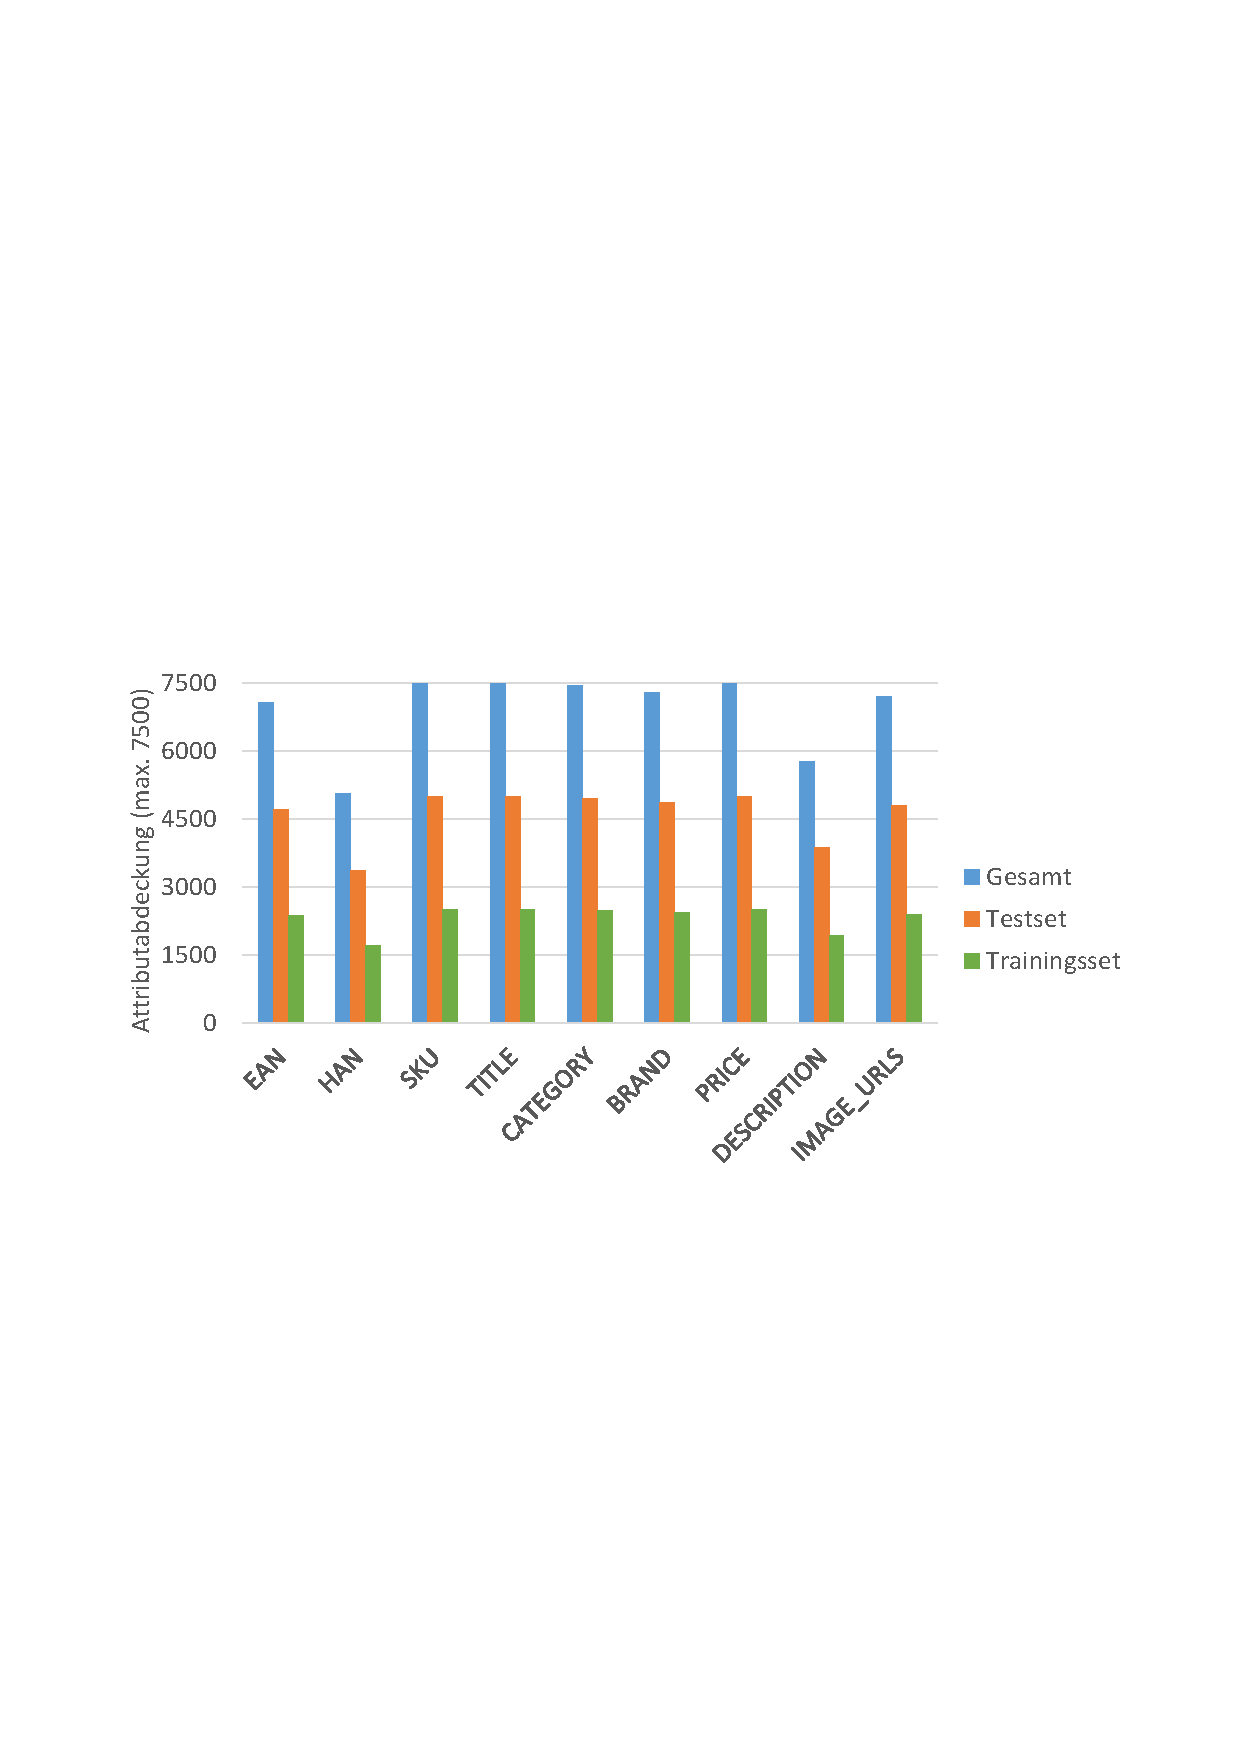
\includegraphics[width=\textwidth, trim=0 10cm 0 11cm, clip]{resources/Testdaten-Attributverteilung.pdf}
    \caption{Attributabdeckung der idealo-Daten, welche für die Evaluierung genutzt wurden}
    \label{abb:testdaten}
    \vspace{-0.5cm}
\end{figure}

Eine Analyse der gesamten Testdaten hat ergeben, dass für jedes Angebot die Angaben zum Titel, dem Preis und der SKU
existieren.
Am seltensten existieren hingegen die HAN (68\%) und die Produktbeschreibung (77\%) eines Angebots.

Das Verhältnis der fehlenden zu den vorhandenen Produktattributen der Trainingsmenge ähnelt dem Verhältnis der
Testmenge und weicht um maximal 0.88\% bei der Produkteigenschaft ``Marke'' ab.

\subsection{Die Messergebnisse}
\label{subsec:genauigkeitsmessung}

Für jeden Shop wurden 21 Regelmengen basierend auf der Trainingsmenge erzeugt, welche sich aus der Kombination
verschiedener Konfigurationen von der Größer der Anlernmenge $SaS$ und dem Filterschwellwert $F$ ergeben.

In allen Statistiken wurden die Fälle ignoriert, bei denen idealo keine Produktattribute gespeichert hat.
Für diese 3440 Fälle ist es unmöglich zu entscheiden, ob die extrahierten Angebotsinformationen korrekt sind.

Die Bestimmung der Genauigkeit erfolgte durch die Anwendung aller Regelmengen auf die Testmenge.
Anschließend wurde ausgewertet, wie oft der extrahierte Wert dem von idealo entspricht.
Zudem wurde für die Bestimmung der Precision erfasst, ob der Wert leer ist.
In \textsc{Tabelle}~\ref{tab:accuracy-precision} sind die typischen Kennziffern Accuracy und Precision für die
verschiedenen Konfigurationen basierend auf den Angeboten aller Shops aufgeführt.

\begin{table}[h]
    \centering
    \begin{tabular}{ c | c c c | c c c }
        &   \multicolumn{3}{c}{\textit{Accuracy in \%}}    &   \multicolumn{3}{c}{\textit{Precision in \%}} \\
        \textbf{F\textbackslash SaS} & \textbf{10} & \textbf{20} & \textbf{50} & \textbf{10} & \textbf{20} & \textbf{50}  \\
        \hline
        \textbf{0}       &   50.59 &   50.78 &   51.07         &   72.73 &   70.81 &   69.62 \\
        \textbf{0.5}     &   52.12 &   53.50 &   \textbf{53.98}&   88.66 &   90.39 &   91.22 \\
        \textbf{0.6}     &   51.87 &   53.07 &   53.15         &   94.15 &   94.03 &   94.93 \\
        \textbf{0.7}     &   50.15 &   51.37 &   52.02         &   96.15 &   96.39 &   95.86 \\
        \textbf{0.8}     &   47.92 &   49.69 &   50.05         &   97.84 &   97.81 &   97.76 \\
        \textbf{0.9}     &   44.61 &   46.92 &   46.57         &   98.16 &   98.14 &   98.42 \\
        \textbf{1.0}     &   41.48 &   39.27 &   36.00         &   98.17 &   97.64 &   \textbf{98.90}

    \end{tabular}
    \caption{Accuracy und Precision bei unterschiedlichen Konfigurationen unter Berücksichtigung der gesamten
    Angebotsmenge aller Shops}
    \label{tab:accuracy-precision}
    \vspace{-0.5cm}
\end{table}

Wie nehmen an, dass für die Matcher-Komponente aufgrund des ähnlichkeitsbasierenden Vergleichs eine höhere Accuracy
wichtiger ist als eine hohe Precision.
Die für unseren Anwendungsfall besten Ergebnisse werden somit für die Parameter $SaS = 50$ und $F = 0.6$ erreicht.

Um eine genauere Aussage zur Precision treffen zu können, wurden alle Nichtübereinstimmungen gesammelt und deren
Levenshtein-Distanz zum erwarteten Wert von idealo berechnet.
Ca. die Hälfte der Nichtübereinstimmungen weisen eine Levenshtein-Distanz $\leq 3$ zum erwarteten Wert von idealo
auf und sind somit ähnlich.
In Tabelle~\ref{tab:levenshtein-examples} sind Beispiele für solche Nichtübereinstimmungen gegeben.

\begin{table}[h]
    \centering
    \begin{tabular}{ p{2.75cm} | p{4.5cm} | p{4.5cm} | p{1cm}}
        \textbf{Produkt-eigenschaft} & \textbf{extrahierter Wert} & \textbf{erwarteter Wert} &
        \textbf{Distanz} \\
        \hline
        TITLE & KENZO LELIXIR & KENZO L'ELIXIR & 1\\
        PRICE & 22642 & 22644 & 1\\
        DESCRIPTION & Objektiv, für Canon; EF	& Objektiv, für Canon, EF & 1\\
        BRAND &	kuechenprofi & Küchenprofi & 2\\
        BRAND & jack-wolfskin & Jack Wolfskin & 3\\
        BRAND & allcare & All Care & 3
    \end{tabular}
    \caption{Nichtübereinstimmungen, welche eine Levenshtein-Distanz $\leq 3$ besitzen}
    \label{tab:levenshtein-examples}
    \vspace{-0.25cm}
\end{table}

Der Tabelle kann man entnehmen, dass oftmals Kodierungsfehler oder unterschiedliche Trennzeichen eine
Übereinstimmung verhinderten.
Außerdem war es häufiger der Fall, dass der Preis um wenige Centbeträge von der Momentaufnahme der idealo-Daten
abwich.
\newpage
Eine nähere Betrachtung der Kennziffern je Attribut liefert \textsc{Abbildung}~\ref{abb:accuracy-precision-chart}.

Wie erwartet, wird die Produktbeschreibung und die Kategorie selten extrahiert.
Dies hängt damit zusammen, dass diese Informationen am stärksten von idealo manipuliert werden.
Interessanterweise wird die HAN ebenfalls selten extrahiert, was mit dem häufigen Fehlen der HAN in den
Testdaten zusammenhängt.

Die in der Bild-URL enthaltene ID und die Marke werden häufig gefunden und könnten somit nützliche Features
für den maschinenlernbasierten Vergleich des Matchers sein.

\begin{figure}[H]
    \centering
    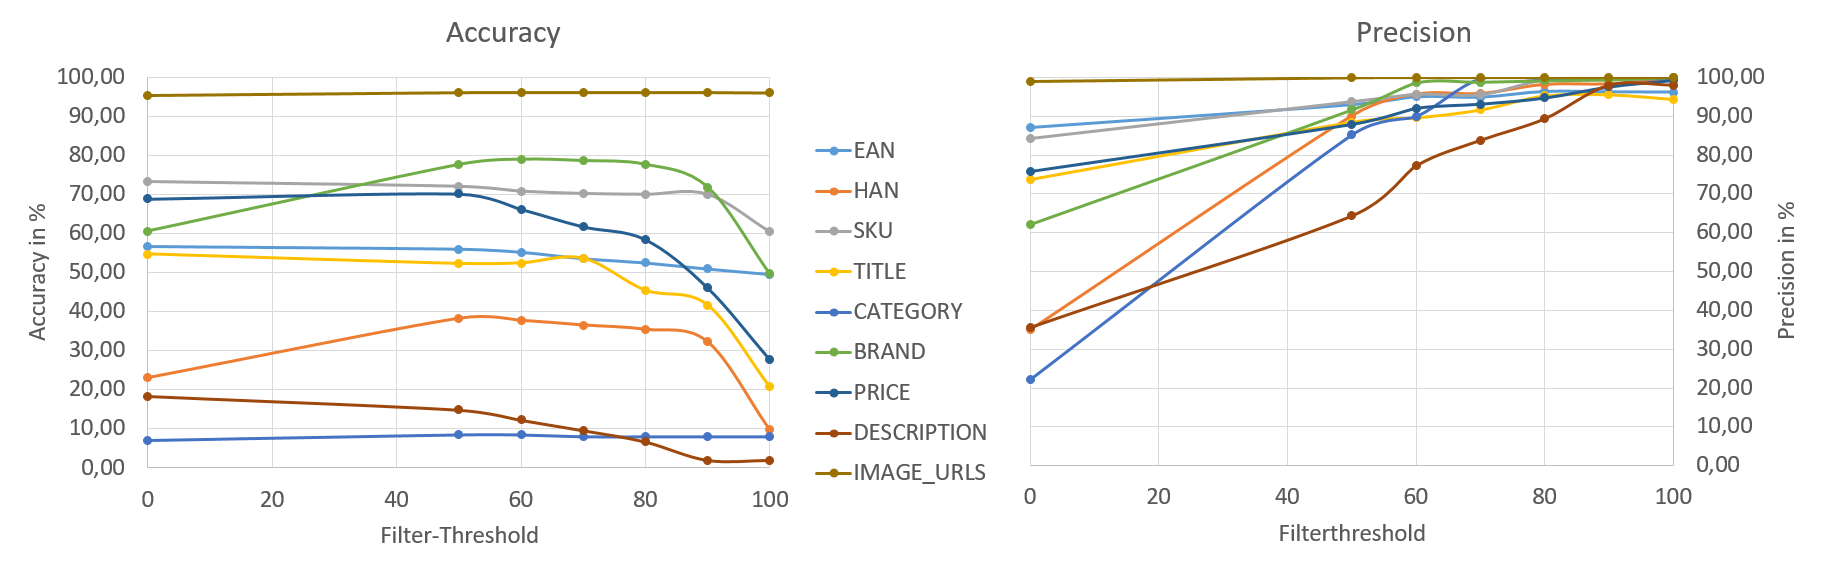
\includegraphics[width=\textwidth]{resources/accuracy-and-precision-per-attribute.PNG}
    \caption{Accuracy (links) und Precision (rechts) pro Attribut für $SaS=50$}
    \label{abb:accuracy-precision-chart}
    \vspace{-0.5cm}
\end{figure}

Zu guter letzt kann man dem Diagramm entnehmen, dass der Filterschwellwert ein gutes Mittel ist, um die Accuracy und
Precision zu beeinflussen und ein höherer SaS-Wert tendenziell besser ist.
Je höher der SaS-Wert gewählt wird, desto höher ist die Accuracy und Precision.
Mit zunehmenden Filter-Schwellwert $F$ sinkt die Accuracy, jedoch steigt dafür die Precision der extrahierten Attribute.

In der \textsc{Abbildung}~\ref{abb:accuracy-precision-box-plot} ist für die gewählten Parameter $SaS=50$ und $F=0.6$
die Streuung der Accuracy und Precision abgebildet.
\begin{figure}[h]
    \centering
    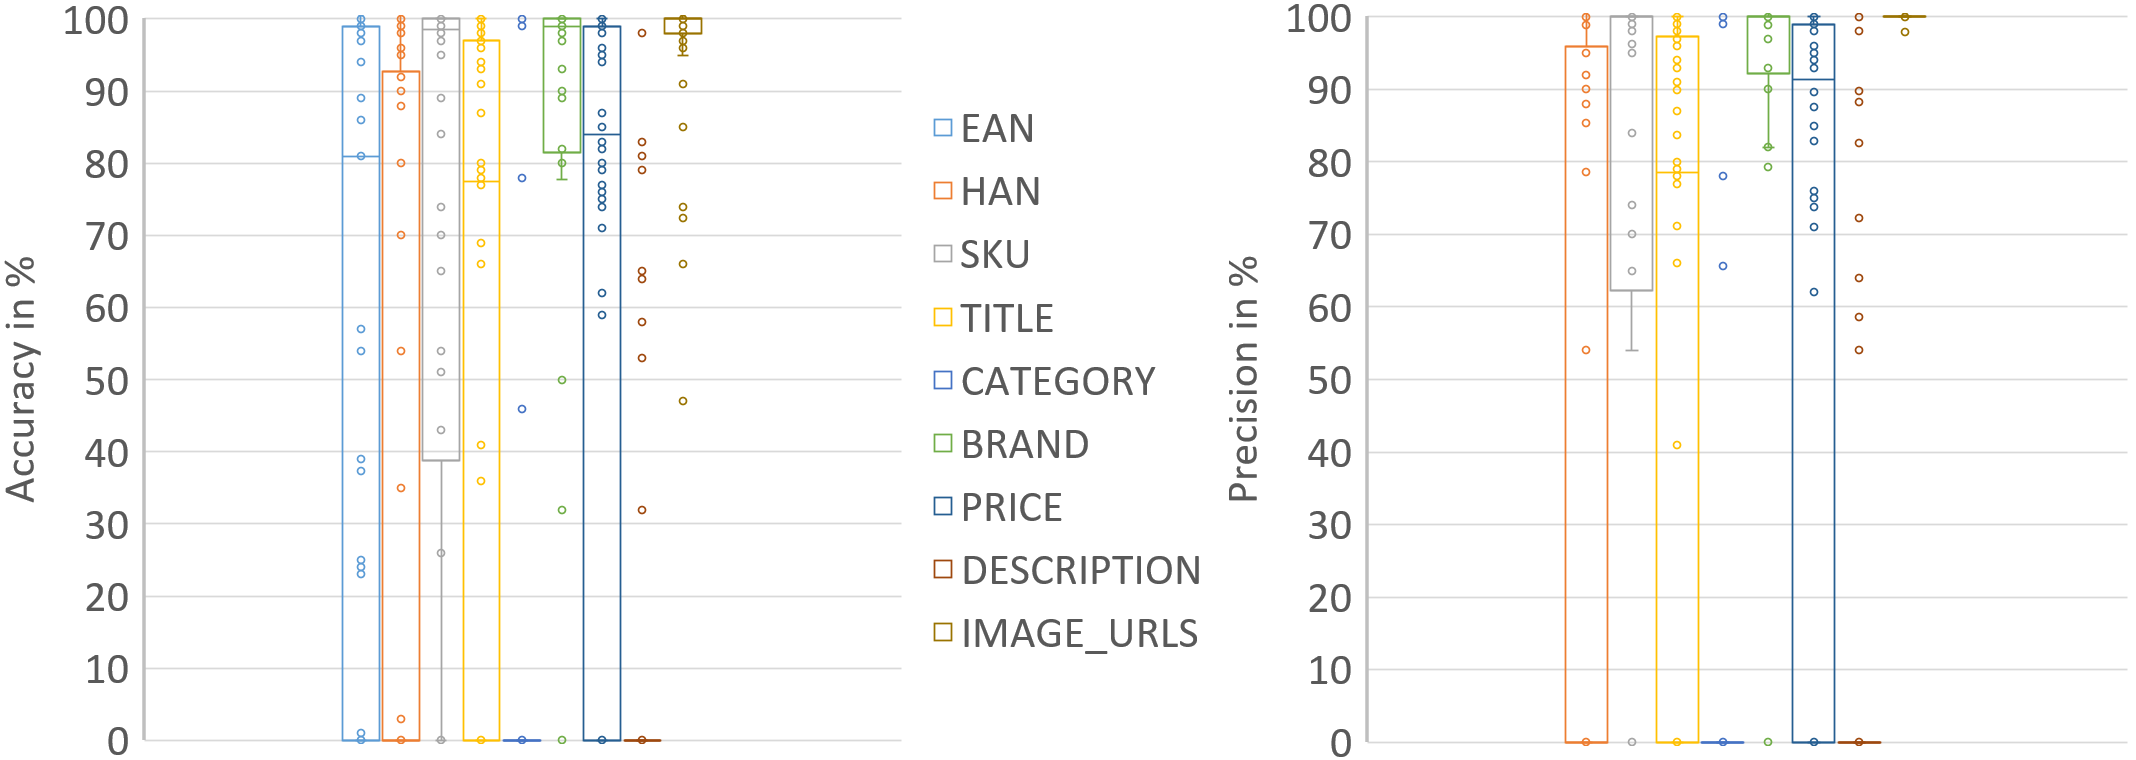
\includegraphics[width=0.95\textwidth]{resources/accuracy-and-precision-box-plots.png}
    \caption{Accuracy (links) und Precision (rechts) pro Attribut für $SaS=50$ und $F=0.6$}
    \label{abb:accuracy-precision-box-plot}
    \vspace{-0.25cm}
\end{figure}
Den Diagrammen kann man zum einem entnehmen, dass es zwar einige Ausreißer gibt, zum anderen wird noch einmal
deutlich, dass die Marke, der Bildlink sowie die SKU häufig und genau extrahiert werden.
Die Shops, welche stark vom angezeigten Median abweichen, könnten ein guter Anhaltspunkt für zukünftige Verbesserungen
der Parser-Komponente sein.
\vspace{-0.25cm}
\subsection{Mögliche Fehlerquellen der Messungen}
\label{subsec:fehlerquellen}

Die getroffenen Annahme, dass die idealo-Daten nicht von denen der Shops abweichen, trifft in der realen Welt nicht zu.
Die Angebotsdaten werden von idealo teilweise manuell oder durch Normalisierungsprozesse manipuliert.
Dadurch können zum Beispiel korrekt extrahierte Produktattribute fälschlicherweise als inkorrekt markiert werden.
Außerdem wird durch wird die Abweichungen die Regelgenerierung erschwert.
    \newpage
    \section{Das Fazit und der Ausblick}
\label{sec:abschluss}

Der Preisvergleich ist ein wichtiges Instrument, um die Markttransparenz im Internet zu gewährleisten.
Damit ein möglichst objektiver Preisvergleich sichergestellt werden kann, ist es erforderlich, einen annähernd
vollständigen Angebotskatalog zu vergleichen.
Das Ziel des Softwaresystems \textit{Scout} ist es, die Vollständigkeit des idealo-Angebotskatalogs zu untersuchen.

Für das Erfassen aller Produkte eines Onlinehändlers stellt die Datenextraktion einen wichtigen und schwierigen
Schritt dar.
Zur Lösung dieses Problems haben wir eine shop-spezifische Lösung entwickelt.
Die Evaluierung hat ergeben, dass der Algorithmus je nach Anwendungsfall eine hohe Präzision erreichen kann.
Auf den Testdaten von idealo wurde beispielsweise zwar nur jedes zweite Attribut gefunden, dafür jedoch auch eine
Präzision von über 95\% erreicht.
Die Ergebnisse können nun von der Matcher-Komponente des Softwaresystems Scout für den ähnlichkeitsbasierten
Vergleich verwendet werden.
\\
~\\
Das Projektpartner idealo ist bereits aktiv dabei, die implementierte Lösung aktiv in deren System zu
integrieren und weiter zu verbessern.
Für die zukünftige Weiterentwicklung besteht noch Potenzial bei der Entwicklung weiterer Selektoren, damit der Parser
weniger von der konkreten HTML-Struktur abhängig ist.
Des Weiteren kann man untersuchen, ob die Qualität der Selektoren durch eine gezielte Auswahl der Angebote, welche
für das Anlernen verwendet werden, verbessert werden kann.
Die Struktur von Shops kann sich unter Umständen innerhalb eines bestimmten Zeitraumes ändern.
Eine mögliche Lösung hierfür wäre zum Beispiel die Einführung einer \textit{Lebensdauer} für Regeln, damit diese nach
einer bestimmten Zeit neu generiert werden.
Abschließend kann man das Anlernen weiter verbessern, indem man die Normalisierungen der Angebotsdaten von idealo
rückgängig macht und an das Format der Shops anpasst.
Ein konkretes Beispiel wäre für den Preis nicht nur nach 12,00€ zu suchen, sondern auch nach 12,0€.
    \newpage

    \bibliography{main}
    \bibliographystyle{plaindin}      % BibTeX Styles nach Norm DIN 1505

\end{document}
